\documentclass[../main.tex]{subfiles}

\begin{document}

To take a deeper look at why the generic one dimensional bootstrap particle filter of \autoref{sec:generic_bootstrap_pf} performs badly at tracking the underlying price state, we use a dataset consisting of 60 minutes of high frequency tick data for the EUR/USD currency pair from the 16th of October 2019, totalling 4196 discrete price observations. 

Figure \ref{fig:4__1__1__bootstrap_PF} gives both the observed and inferred returns and price process for the simple bootstrap particle filter. We can clearly see the effectiveness of the noise removal in the inferred returns process. However, we note that the inferred price process suffers greatly from drift. Small errors in the inference of the returns process are compounded, leading to the inferred price process deviating from the observed price. 

This causes the poor inference results when the generic particle filter is used to infer the underlying price process of the simulated signal in Figure \ref{fig:4__1__comparison_price}.

\begin{figure}[h!]
	\centering
	\subfloat[Inferred Returns Process \label{fig:4__1__1__bootstrap_naiive}]{
		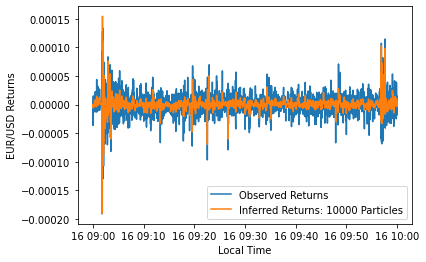
\includegraphics[height=4.5cm]{../plots/4__1__1__bootstrap_naiive.png}}
	\qquad
	\subfloat[Inferred Price Process \label{fig:4__1__1__bootstrap_naiive_price}]{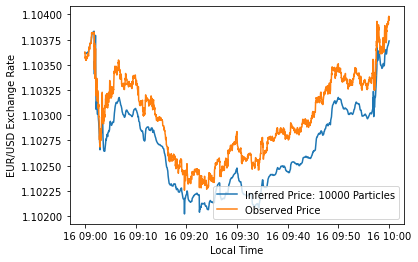
\includegraphics[height=4.5cm]{../plots/4__1__1__bootstrap_naiive_price.png}}
	\caption{Simple Bootstrap Particle Filter, $N = 10000$ particles}
	\label{fig:4__1__1__bootstrap_PF}
\end{figure}

On the other hand, the drift-corrected particle filter attempts to correct for price drift in the system by using numerical integration to obtain an estimate of the current inferred value of the price process at every time step. 

Figure \ref{fig:4__1__1__drift_corrected} gives both the observed and inferred returns and price process for the drift-corrected particle filter. We note qualitatively that the inferred returns process shows much greater noise reduction, and the inferred price process no longer suffers from price drift. 

\begin{figure}[h!]
	\centering
	\subfloat[Inferred Returns Process \label{fig:4__1__1__drift_corrected}]{
		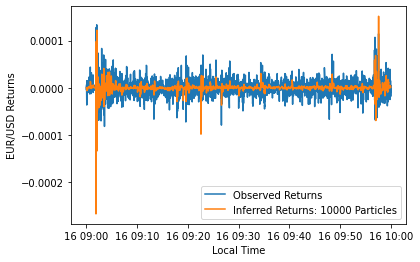
\includegraphics[height=4.5cm]{../plots/4__1__1__drift_corrected.png}}
	\qquad
	\subfloat[Inferred Price Process \label{fig:4__1__1__drift_corrected_price}]{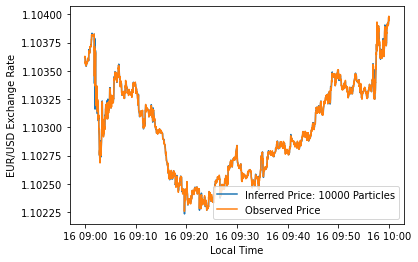
\includegraphics[height=4.5cm]{../plots/4__1__1__drift_corrected_price.png}}
	\caption{Drift-Corrected Particle Filter, $N = 10000$ particles}
	\label{fig:4__1__1__drift_corrected_PF}
\end{figure}

\end{document}

